\section{Method}

% balance goes out the window with great flowers - no normalization.

\subsection{Motivation}

We seek a function that is uniquely minimized by unitary matrices.
While operator norm, also known as deformation, is the fraction of the largest and smallest singular values, it does not take into account variability along different axes.
This could be an issue in high dimensional situations.

\subsection{Normalization}

Since basis pursuit methods tend to select longer vectors, selection of unitary submatrices requires normalization such that long and short candidate basis vectors are penalized.
We establish some basic conditions for vector normalization.
\begin{definition}[Symmetric normalization]
A function $q: \mathbb R^D \to \mathbb R^+ $ is a symmetric normalization if 
\begin{align}
\arg \max_{v \in \mathbb R^D} \ q (v) = v \; \|v\| = 1 \\
q(v) = q(\frac{v}{\|v\|^2}) \\
%q convex?
\end{align}
\label{cond:normalization}
\end{definition}

Thus, let
\begin{align}
\label{eq:normalization}
q: \mathbb R^+ \times \mathbb R^+  &\to \mathbb R^+ \\
t , c &\mapsto \frac{\exp(t^c) + \exp(t^{-c})}{2e},
\end{align}
and use this to define the normalization 
\begin{align}
n: \mathbb R^D \times \mathbb R^+ &\to \mathbb R^D \\
n^d , c &\mapsto \frac{n^d}{q(\|n\|_{2},c) } \forall d \in [D].
\end{align}

This normalization scales lengths down that are far away from $1$ is a logarithmically symmetric way.
Any rescaling which is maximized at $1$ and logarithmically symmetric satisfies Proposition \ref{prop:main}, but $n$ is particularly suitable.
First, $q$ is convex.
Second, it grows asymptotically log-linearly.
Third, while $\exp(-|\log t|) = \exp(-\max (t, 1/t))$ is a seemingly natural choice for normalization, it is non smooth, and the LogSumExp replacement of $\max (t, 1/t)$ with $ \log (\exp (t ) + \exp(1/t))$ simplifies to \ref{eq:normalization} upon the exponentiation.
% Introduce the exponent here.
Finally, the parameter $c$ grants control over the width of the basin, which is important in avoiding numerical issues arising close to $0$ and $\infty$.

\begin{figure}[htbp]
    \centering
    \begin{minipage}{0.49\textwidth}
        \centering
        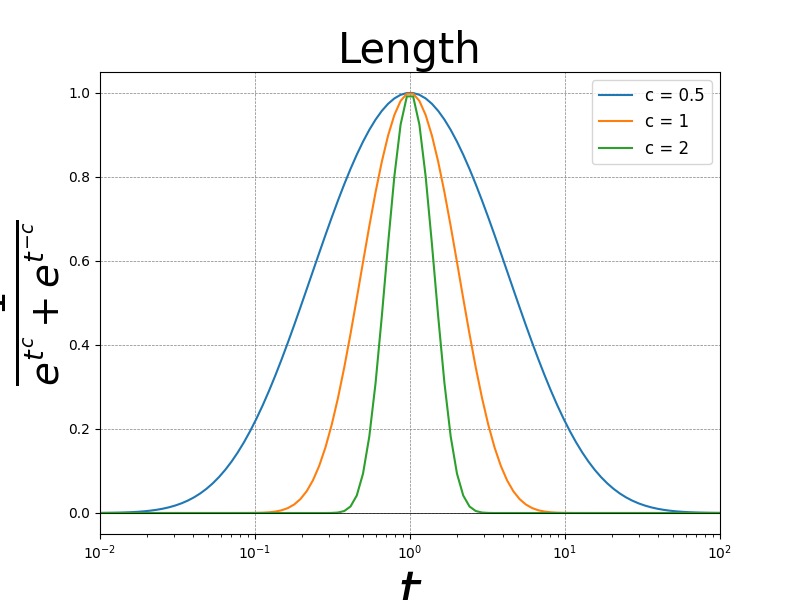
\includegraphics[width=\textwidth]{../figures/Figure_1a.png}
        \caption{Length as a function of $t$}
        \label{fig:length}
    \end{minipage}
    \hfill
    \begin{minipage}{0.49\textwidth}
        \centering
        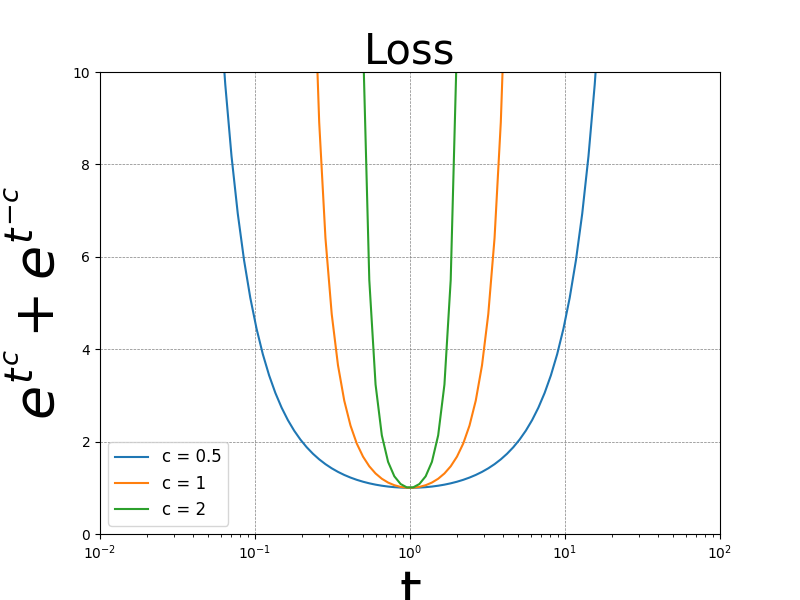
\includegraphics[width=\textwidth]{../figures/Figure_1b.png}
        \caption{Loss as a function of $t$}
        \label{fig:loss}
    \end{minipage}
    \caption{Plots of Length and Loss for different values of $c$}
    \label{fig:results}
\end{figure}


Using this, define the matrix-wide normalization vector
\begin{align}
\mathcal D: \mathbb R^{D \times P} \times \mathbb R^+ &\to \mathbb R^P \\
\mathcal X_{.p}, c &\mapsto n(\mathcal X_{.p}, c)
\end{align}
and the normalized matrix $\tilde {\mathcal X}_c = \mathcal X \mathcal D(\mathcal X, c).$
This completes the data preprocessing.

\subsection{Ground truth}

The main goal of sparse isometry pursuit is to expediate the selection of unitary submatrices.
Typically, unitaryness is measured using the singular values of the matrix.
However, measures like the operator norm and deformation compare only the largest an smallest singular values.
Compared with the nuclear norm, it is symmetric around 1 \cite{Fazel2001ARM}. % is our loss self-dual?
That is, they do not account for the whole spectrum.

Define the loss
\begin{align}
l_{iso}: \mathbb R^{D \times P} \to \mathbb R^{+} \\
\mathcal (X) \mapsto \sum_{d = 1}^D g(\sigma^d(\mathcal X))
\end{align}
where $\sigma^d (\mathcal (X))$ is the $d$-th singular value of $\mathcal X$.
%Note that since $g$ is convex, we could compute a full realization of the convex isometry pursuit algorithm by minimizing over WHAT.
However, this would not result in a sparse solution.

This loss is an appropriate choice for comparison because it is equal to the basis pursuit loss for orthogonal matrices
\begin{proposition}
\label{prop:main}
\end{proposition}
\begin{proof}
\begin{align}
\end{align}
Then, singular values and regressands are analytically determined.  cont.
\end{proof}

\subsection{Isometry pursuit}

Define the multitask group basis pursuit penalty % is this really a norm?
\begin{align}
\label{eq:bp}
\| \cdot \|_{1,2}: \mathbb R^{P \times D} &\to \mathbb R^+ \\ 
\beta &\mapsto  \sum_{p=1}^P  \|\beta_{p.}\|_2.
\end{align}

The isometry pursuit program is then
\begin{align}
\label{prog:isometry_pursuit}
\hat {\beta_{P}} (\mathcal X)  = \arg \min_{\beta \in \mathbb R^{P \times D}} \| \beta \|_{1,2} \; s.t. \; I_D = \tilde{ \mathcal X}_c \beta.
\end{align}
The intuition is that vectors which are closer to 1 in length and more orthogonal will be smaller in loss.

%Direct minimization of Equation \ref{eq:bp} will not select for isometry due to the preference for columns with larger norm.

%One immediate question is - why $\beta$?  Can we just minimize some function of $X$ directly like $\|\exp_1 X\|_{1,2}$?  Direct minimization of this norm has nothing to do with correlation. We wouldn't need orthogonality - just constant length!

\subsection{Isometric lasso}

By Lagrangian duality, define an extension of \ref{prog:ip} called Isometric Lasso.
The Isometric Lasso loss is
\begin{align}
\end{align}
Isometric Lasso is
\begin{align}
l_\lambda (\mathcal X, \beta) =  \|I_D -  \tilde{ \mathcal X}_c \beta\|_2^2 +  \lambda \| \beta \|_{1,2}
\end{align}
which can be optimized as
\begin{align}
\label{prog:isometric_lasso}
\hat {\beta_{\lambda}} (\mathcal X) = \arg \min_{\beta \in \mathbb R^{P \times D}} l_\lambda (\mathcal X, \beta)
\end{align}
The recovered supports are then given by $S(\hat {\beta_{\lambda}} (\mathcal X))$ where 
\begin{align}
S: \mathbb{R}^{p \times d} &\to \binom{\{1, 2, \ldots, P\}}{d} \\
\beta &\mapsto \left\{ p \in \{1, 2, \ldots, P\} :  \|\beta_{p.}\| > 0 \right\}
\end{align}
and $\binom{\{1, 2, \ldots, P\}}{d} = \left\{ A \subseteq \{1, 2, \ldots, P\} : \left|A\right| = d \right\}$ are the indices of the dictionary elements with non-zero coefficients.

\subsection{Theory}
\label{sec:theory}

A key theoretical assertion is that selection methods $S(\widehat {\beta}_{\lambda} (\mathcal X))$ and $S(\widehat {\beta} (\mathcal X))$ are invariant to choice of basis for $\mathcal X$.

\begin{proposition}[Basis pursuit selection equivalence]
\label{prop:basis_pursuit_selection_equivalence}
Let $U \in \mathbb R^{D \times D}$ be unitary.
 Then $S(\widehat \beta  (U \mathcal X)) = S(\widehat \beta (\mathcal X))$.
\end{proposition}

\begin{proposition}[Lasso selection equivalence]
\label{prop:lasso_selection_equivalence}
Let $U \in \mathbb R^{D \times D}$ be unitary.
 Then $S(\widehat \beta_{\lambda}  (U \mathcal X)) = S(\widehat \beta_{\lambda} (\mathcal X))$.
\end{proposition}

%It also may be possible to argue the basis pursuit invariance from the lasso ones plus Lagranian duality, but to avoid taking the limit we prove both propositions  independently.
%This also covers changing the target variable.

With these preliminaries, we may state our main result.

\begin{proposition}[Unitary selection]
\label{prop:unitary_selection}
Given a matrix $\mathcal X \in \mathbb R^{D \times P}$ with a rank $D$ submatrix $\mathcal X_{.\mathcal S} \in \mathbb R^{D \times D}$ that is unitary, $\mathcal S = S(\widehat{\beta} (\mathcal X)))$
%Program \ref{prog:isometry_pursuit} selects $\mathcal S \subset [P]$ with $|\mathcal S| = D$ such that $X_{. \mathcal S}$
 \end{proposition}
 
 A proof is given in Section 
 
This proof admits two immediate generalizations.
First, any normalization function that satisfies the normalization conditions will do.
Second, the ground truth and convex losses are equivalent for diagonalizable matrices.
 %Convex functions form metric? Cite Koelle neuroscience? Is metric important?
 
\begin{proposition}[Local isometry selection]
\label{prop:local_isometry}
Given a set of functions $G$ that contains a subset that defines a locally isometric embedding at a point $\xi$, then these will be selected as $\arg \min_\beta$.
\end{proposition}
A proof is given in Section \ref{sec:local_isometry_proof}.


Algorithm (Local tangent Space basis pursuit)

Algorithm (Local two stage tangent space basis pursuit)

This provides an approach for the problem put forward in (cite) LDLE paper.

Experiments (Loss)

Compare with isometry loss (2 norm of singular values).

\subsection{Implementation}

We use the multitask lasso from sklearn and the cvxpy package for basis pursuit.  We use the SCS interior point solver from CVXPY, which is able to push sparse values arbitrarily close to 0 \cite{cvxpy_sparse_solution}. Data is IRIS and Wine, as well as flat torus from ldle.
\subsection{Computational complexity}
\section{Experiments}

Comparison with isometry loss.